\documentclass[../draft_1.tex]{subfiles}

\begin{document}

\chapter{Cardiac Electrophysiology}

Our hearts are absolutely vital for our survival. While it normally functions with an incredible reliability and accuracy that does not even let us begin comprehend the complexity of the mechanisms involved, cardiovascular diseases are estimated to make up for more than 30\% of all world wide's death \cite{WHO_statistics}. Often this is related to abnormal heart contractions and thus understanding the processes involved in governing our heart beats is crucial to explaining heart failues. The heart acts as a double pump made out of muscle tissue that provides our bodies with freshly oxygenated blood \cite{deMotuCordis}. A heart has about the size of a fist and sits between our two lungs. It consists of 4 chambers, the upper two atria, that is the left and right atrium and the lower two ventricles which have connections through four heart valves that can open and close respectively but only allow the blood to flow in one direction. The left and the right side of the heart is separated by a wall of tissue known as the atrioventicular septum. An intricate interplay of contraction and relaxation of the chambers governed through electrical stimuli lead to a stable blood flow that enables the replenishment of oxygen levels of the cells in our body. Below we can see a schematic image of the heart, where the arrows indicate the direction of blood flow.

\begin{figure}[ht!]
	\centering
	%\includegraphics[scale=0.2]{images/heart_structure}
	\includegraphics[scale=0.3]{images/electrophysiology/heart_structure}
	\caption{Scheme of the Heart \cite{franzone2014mathematical}}
\end{figure}

The blood flow through the different chambers of the heart occurs in repeating cycles. After circulating through the body low oxygenated blood flows back into the heart through our veins and enters into the right atrium, which contracts once it is full. This contraction causes a pressure built up and pushes the tricuspid valve open. The blood rushes into the right ventricle, whose walls, once filled, also begin to contract, the pressure within rises again, which shuts tricuspid valve and opens the pulmonary valve to the pulmonary artery from where the blood reaches the lungs and replenishes it oxygen stocks. Afterwards it returns to the left side of the heart from the pulmonary veins to the left atrium, which again, once it is completely filled, contracts and hereby opens the miral valve and forces the blood into the left ventricle. The left ventricle then pumps the oxygenated blood through the aortic valve into the aorta from where it flows into different parts in the body to supply cells with oxygen and nutrients before returning to the right atrium and repeating its cycle. The mitral and tricuspid valves open, and the aortic and pulmonic vavles close while the ventricles fill with blood. In contrast the mitral and tricuspid valves shut, and the aortic and pulmonic valves open during ventricular contraction. This particular sequence makes sure that all ventricles are filled up to capacity before pumping and that blood flows only in one direction. For references and further information see \cite{cardiosmart}, while the following sections are based on \cite{franzone2014mathematical}.
\bigskip
\\ 
\begin{figure}[ht!]
	\centering
	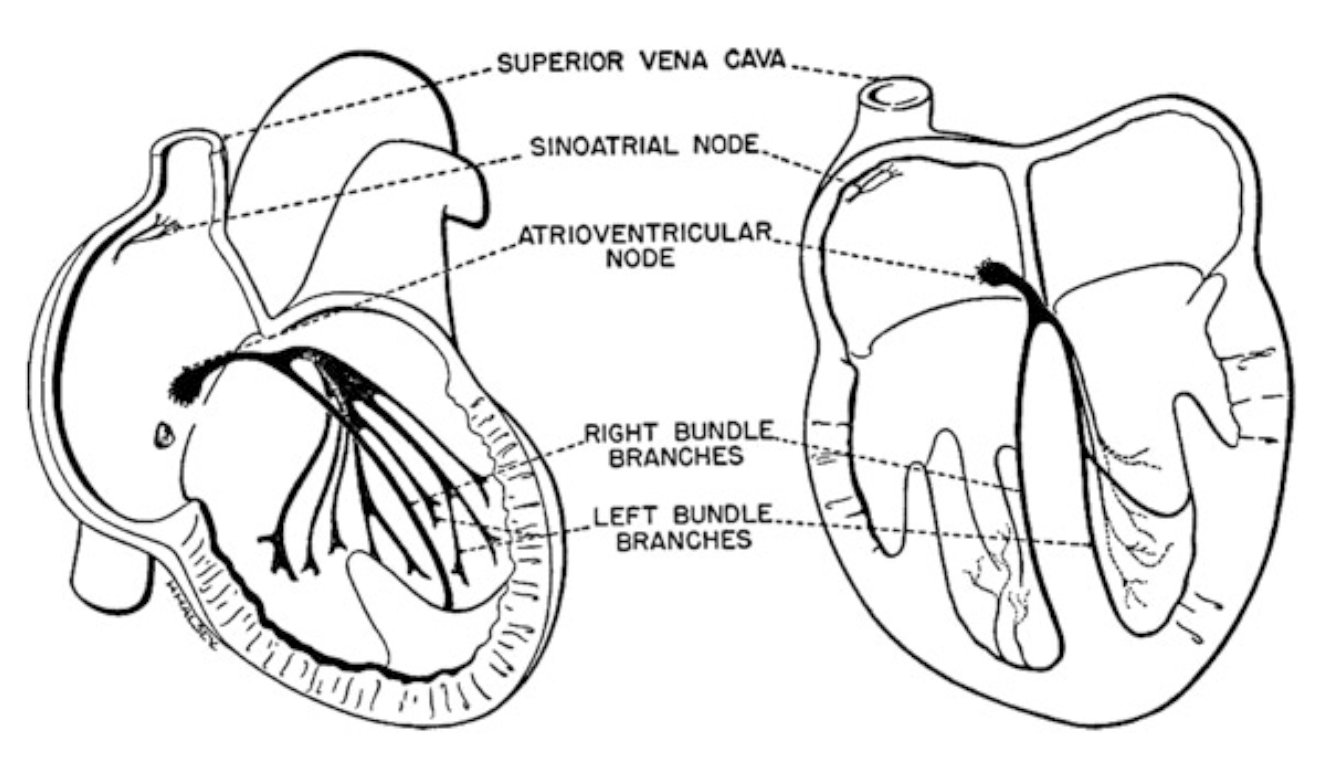
\includegraphics[scale=0.5]{images/electrophysiology/conduction_system}
	\caption{Overview of the Hearts Conduction System \cite{franzone2014mathematical}}
\end{figure}

The heart contractions are initiated by an electric activiation, that is a depolarizing transistory membrane current which raises the transmembrane potential from its resting value of about -90 to -80 mV to small positive values. This potential describes the difference in the electric potential between the interior and exterior of the cell. The increase is followed by a repolarization current which sends the transmembrane potential back to its resting value. The initial electrical stimulus is generated by the sinoatrial node which is located on the right atrium close to the superior vena cava and possesses the ability to excite its cells autonomously. The frequency of its stimuli is dependent on the parasympathetic nervous system and hormonal factors but under normal health and stress conditions ranges from about 60-100 times per minute. The signal is then transmitted through the surrounding cells and cardiac conduction pathways to the various chambers of the heart. It first propagates to the right atrium and through Bachmann's bundle to the left atrium where it stimulates the cardiac muscle cells of the atria to contract. The activation front then travels to the atrioventricular node situated at the base of the atria. The cells there have a relatively slow conduction velocity and therefore cause a delay in the transmission which is timed this way to achieve optimal pump activity. From the atrioventricular node the stimulus reaches specialised fibres in the bundle of His and the Purkinje network that branch in the left and right bundle onto the inner surface of the ventricals. Again causing a contraction of the cardiac muscle tissue. 

\section{Electrical Activity on the Cellular Level}

The heart's walls can be subdivided into 3 different layers; the inner endocardium which surrounds the the heart chambers; the outer endocardium which protects and delimits the heart from other parts of the body and the predominant middle layer consisting of cardiac muscle tissue called myocardium. This is where the conduction of the electric potential and the heart contractions mainly take place. Myocardium is made up of sheets of cells, where each one is roughly of a cylindrical shape with a size ranging from 100-150 $\mu$m by 30-40 $\mu$m. (diff source 50-150, 10-20) They are organised in a way similar to a brick wall and joined together at the ends by intercalated disks turning them into long fibres. The disks allow for easy ion movement between the cells and thus allowing for a rapid transmission of electrical impulses. Each cardiomyocyte that is each cardiac muscle cell contains bundles of myofibrils which are protein fibres which can slide past each other, making it possible for the tissue to contract. The cell's membrane is called sarcolemma and contains certain transmembrane channels whose opening and closing is governed through electric stimuli (mainly transversal cell direction?). The intercalated disks allow the transit of ions through channels called gap junctions which are predominantly in longitudinal fiber direction. Due to the varying density of the gap junctions in the different directions there is an anisotropic propagation of the electric potential throughout the tissue which complicates its simulation. 

\begin{figure}[ht!]
	\centering
	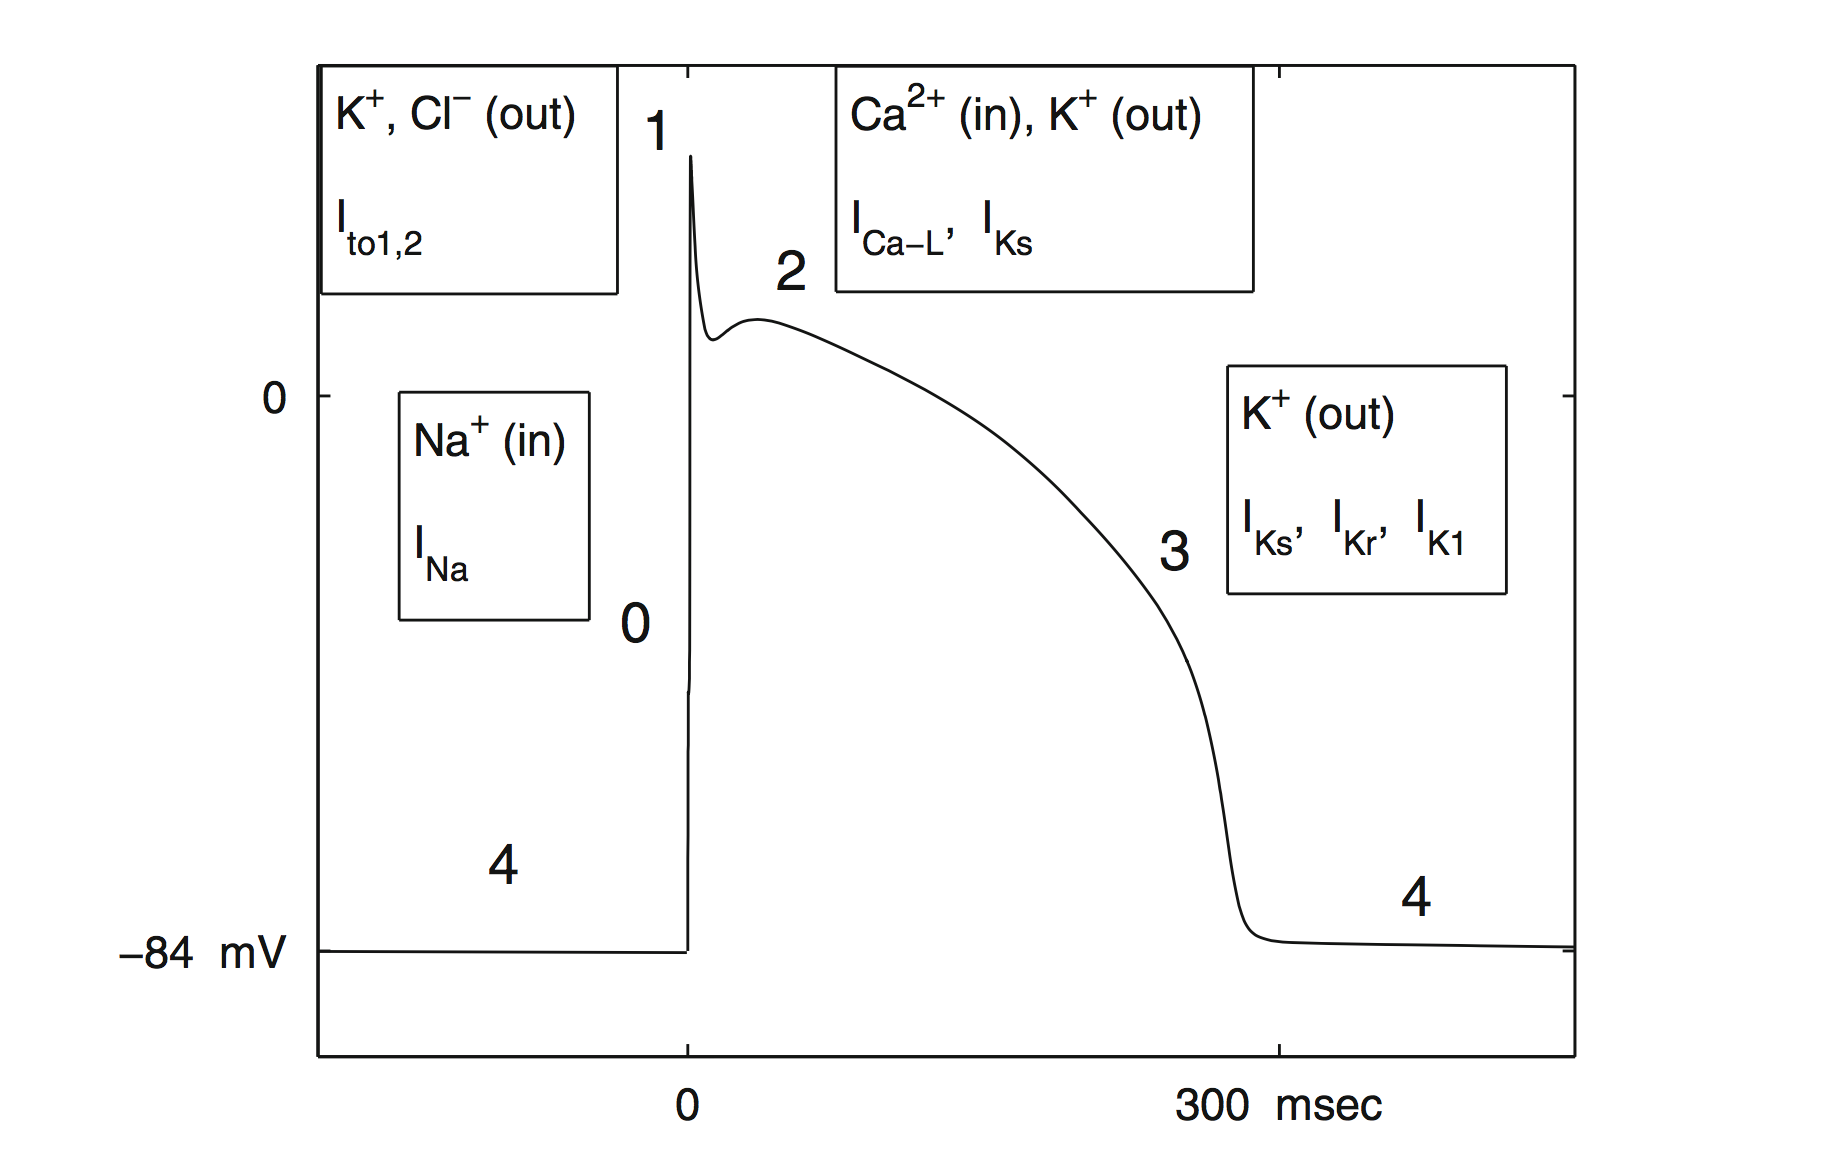
\includegraphics[scale=0.3]{images/electrophysiology/cardiac_action_pot_franzone}
	\caption{Different Phases of Cardiac Action Potential \cite{franzone2014mathematical}}
\end{figure}

In this figure we can see a standard ventricular action potential in its main phases, that is the electric charge distribution a cell goes through over time. Following \cite{franzone2014mathematical} we will have a brief look at the different stages that occur and what they entail.
\smallskip
\\
\underline{Phase 0:} Depolarization of the cell by opening of $Na^+$ channels of the sarcolemma which leads to rapid inflow of $Na^+$ ions into the cell. Hence, the transmembrance potential passes from negative to positive values. \\
\underline{Phase 1:} Outward flow of $K^+$ and $Cl^-$ ions after the inactivaiton of $Na^+$ channels, which causes a rapid decrease of the potential \\
\underline{Phase 2:} Governed by an inward as well as an outward current of $Ca^{2+}$ and $K^+$ ions respectively such that there almost is a balance in the potential \\
\underline{Phase 3:} Repolarization of the cell by closing of the $Ca^{2+}$ channels while outward current of $K^+$ ions is maintained therefore returning the potential to negative values. \\
\underline{Phase 4:} The potential remains at a constant negative value. Some channels are kept open to allow for keeping the right inter-and extracellular charge balance. The cardiomyocyte stays in this resting state until the next stimulation. 
\smallskip
\\
The stimuli are under normal conditions about 0.6-1 seconds apart, which means that the cell is about half the time in its resting phase. They travel as a wave through the cardiac tissue, where one cell excites the next. After this brief description of the processes involved in the functioning of the human heart, let us in the subsequent section turn towards the question of how to adequately represent them in a model and what the particular difficulties are that arise.


\section{The Monodomain Equation}

The propagation of these stimuli is usually modeled with either a version of the bidomain equation or monodomain equation. The former was first developed in the late 1970's and is the more comprehensive one of the two still posing many computational challenges in its implementation and execution. Therefore one often relies on a simpler monodomain model which in the vast majority of applications leads to a very similar solution and can therefore be considered as an adequate approximation, \cite{potse2006comparison}. The discrete cellular structure is replaced by an averaged continuous model, giving rise to a parabolic reaction-diffusion equation derived from the cable equation maintaining a conservation of charge. Cable theory is used to calculate the electric current in nerve fibres by modeling them as composed segments with capacitances and resistences combined in parallel. 
% only have a good picture from wikipedia,  $c_m$,  $r_m$
The diffusion term represents the spread of current through gap junctions and cardiac tissue while the reaction terms describe the flux of ions across the myocyte membrane. \textit{say more about internal and external current.}
\begin{ceqn}
\begin{equation}
\begin{aligned}
\partial_t u - \nabla \cdot ( D(x) \nabla u) &= I_{\text{int}}(u) + I_{\text{ext}}(x,t)  \quad  (x,t) \in \Omega \\
\nabla u \cdot n &= g(x,t) \qquad \qquad \qquad (x,t) \in \Gamma_N \\
\end{aligned}
\end{equation}
\end{ceqn}

where the above terms describe the following 
\smallskip
\\
$u(x,t)$ : electric potential \\
$D(x) $  : conductivity tensor \\
$ I_{\text{int}}(u) $: internal current \\
$I_{\text{ext}}(x,t)$: external current 
\bigskip
\\
In the case of the simplified FitzHugh-Nagumo model we have $I_{\text{int}}= u (u - 1 )(\alpha - u)$, with $ 0 < \alpha < 1$. \textit{mention gating variables...? }
\smallskip
\\
There are a number of difficulties that arise when trying to numerically approximate a solution to this problem. One is the beforementioned challenging task of dealing with large differences in spatial and temporal scaling due to the complex multiscale structure. As mentioned before the microscopic scale the electric conduction of excitation fronts happens through ion channels of cellular membranes which are on a scale of the order of 0.1 mm. On the other hand the overall size cardiac tissues invovled entails a size of several centimeters which leads to a spatial spread factor of up to $10^3$. Similarly for the time parametrisation we have an even larger spread factor. A normal heartbeat takes about 1 second, that is one full cycle, whereas the step excitation front that is described in phase 0 in the previous section ranges on a much shorter time scale therefore requiring time steps within a range of about 0.1 to 500 milliseconds for accurate representation \cite{colli2004parallel}.
\smallskip
\\
But the sheer size of the problem is not the only difficulty, as mentioned in the prologue there are many ways to discretise the domain, various methodologies of how to represent the differential operators and how to approximate the arising linear and nonlinear systems of equations. As we have tried to reason for the particular choices we have made, the following chapter is meant to serve as an introduction to these mathematical methodologies we apply, outline their underlying principles, demonstrate their functioning using standard examples and point out their relevance and applicability for other \textit{problems}.

\end{document}